 \section{Arquitectura de red basada en BUS}\label{sec:bus}
En \cite{Tai99} se presenta una arquitectura tolerante a fallas basada en BUS. Esta topología forma parte de un programa denominado X2000, el cual tiene como objetivo desarrollar una arquitectura tolerante a fallas y basada en componentes COTS, perteneciente a \ac{NASA}. Este programa se desarrolla bajo una filosofía de misiones espaciales la cual dice: ``Rápido, mejor, barato'' \footnote{En ingles, faster, better, cheaper}.

Esta arquitectura utiliza una topología novedosa denominada \textit{stack-tree topology} (\citep{Chau99}; \citep{Tai99}). Una stack-tree es un árbol donde cada nodo rama se encuentra conectado como mucho a tres otros nodos de los cuales, como máximo, dos son nodos ramas \citep{Tai99}. Una \ac{CST} es aquella en donde cada nodo rama está conectado al menos 1 nodo rama \citep{Tai99}.

En las Figura \ref{fig:stack-tree} se pueden observar ejemplos de stack-tree. Mientras que en la Figura \ref{fig:no-stack-tree} no es una stack-tree. Las imágenes fueron extraídas de \cite{Tai99}

\begin{figure}[h]
 \centering
 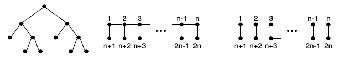
\includegraphics[scale=1]{images/Marco_teorico/stack-tree.jpg}
  \caption{Arquitecturas stack-trees}
\label{fig:stack-tree}
\end{figure}

\begin{figure}[h]
 \centering
 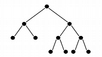
\includegraphics[scale=1]{images/Marco_teorico/no-stack-tree.jpg}
  \caption{Arquitecturas que no responden al modelo stack-trees}
\label{fig:no-stack-tree}
\end{figure}

Como el objetivo principal es desarrollar una arquitectura tolerante a fallas, esto es, que aún cuando un nodo o un link entre nodos falle, el sistema completo debe continuar funcionando, sin ningún tipo de degradación en su servicio. Para cumplir con este objetivo \cite{Tai99} trabajan con un esquema de denominado \ac{CST} de equema dual (\ac{CST}$_D$) \footnote{En ingles,\ac{CST} dual scheme}. Esta puede observarse en la Figura \ref{fig:cstd} extraída de \cite{Tai99}.

\begin{figure}[h]
 \centering
 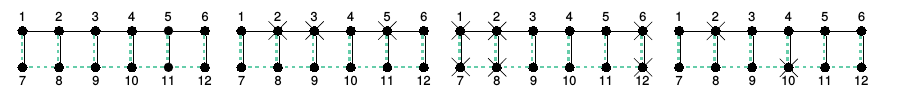
\includegraphics[scale=0.5]{images/Marco_teorico/cstd.png}
  \caption{Esquema CST$_D$}
\label{fig:cstd}
\end{figure}


Para aumentar la confiabilidad de la arquitectura ante la ocurrencia de fallas, se agrega links de backups que unen los nodos iniciales con el final, dando un efecto 3D de anillo \citep{Tai99}.

\subsection{Evaluación de la confiabilidad de arquitecturas basadas en BUS}
La confiabilidad de esta arquitectura (como ya se viene mencionando) es la probabilidad de que, a lo largo del tiempo de vida de la misión $t$, la arquitectura se encuentra funcional, en la cual todos los nodos (aquellos que no hayan fallado) se encuentren conectados \citep{Tai99}.

\cite{Tai99} y \cite{Chau99} asumen que la probabilidad de que un nodo falle es mucho mayor a que un enlace (el bus físico) falle.

\cite{Tai99} indican que la confiabilidad de la red depende del tamaño $k$, siendo $k$ el números de nodos ramas. La confiabilidad de una red basada en \ac{CST} simplex es la probabilidad $U(k)$ de que los nodos no fallen, o que ante una falla, se detecte y se lleve a cabo correctamente la reconfiguración del sistema. $$U(k) = (1-q) \sum_{j=0}^{k} {{k}\choose{j}} (1-q)^{k-j} (cq)^j $$ donde $q = 1-e^{-\lambda t}$ es la probabilidad de que un nodo falle durante el tiempo de vida de la misión $f$. Entonces $$R_s^{CST} = \sum_{k=1}^n (n-k+1)U(k)(cq)^{2(n-k)}$$ donde $(cq)^{2(n-k)}$ es la probabilidad que los  $2(n-k)$ nodos que conforman un cluster fallen, y esta falla es detectada y se lleva a cabo una correcta reconfiguración.

Para un \ac{CST} dual ocurre de manera similar. Se define $V(k)$ de la siguiente manera: $$V(k) = 2(1-q)^k \sum_{j=1}^k {{k}\choose{j}} (1-q)^{k-j} (cq)^q + (1-q)^{2k}$$

Entonces:  $R_D^{CST} =  \sum_{k=1}^n (n-k+1) V(k) (cq)^{2(n-k)}$
